\section{Results}

\subsection{Average funding trends over 2015-2022}

\begin{figure}
    \centering
    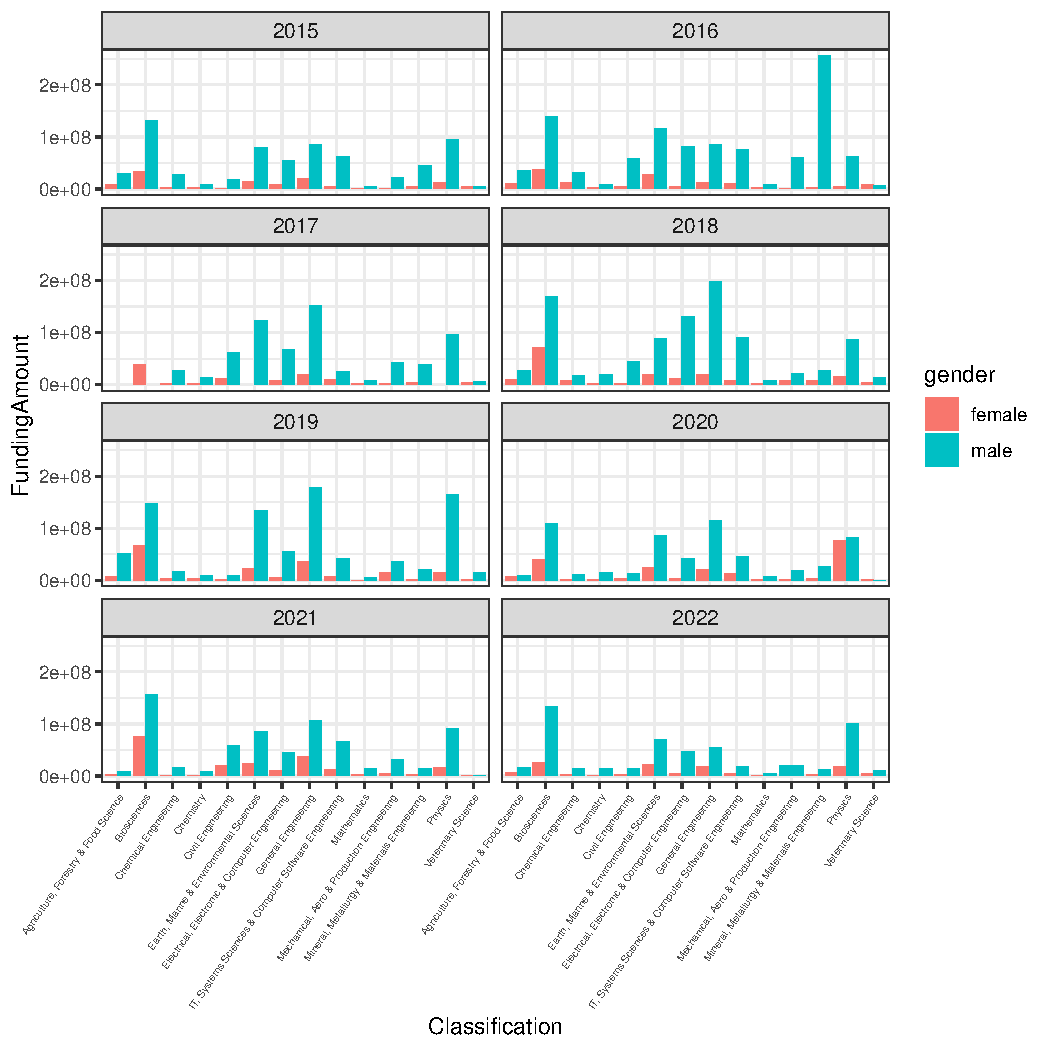
\includegraphics[width = 1\textwidth]{funding_all.pdf}
    \caption{Average research funding allocated to each gender during the period measured. The plot shows a gap in most of the STEM subjects, and that the funding amount for male researchers is generally higher.}
\end{figure}
Figure 1 shows that there is a large gender gap in most engineering-related subjects, except Chemical Engineering, where the gap is rather small. In general, the average funding amount for male researchers is greater than that for female researchers, except in the fields of Physics and Veterinary Science, where the average funding amount for females is larger than that for males.
\begin{figure}
    \centering
    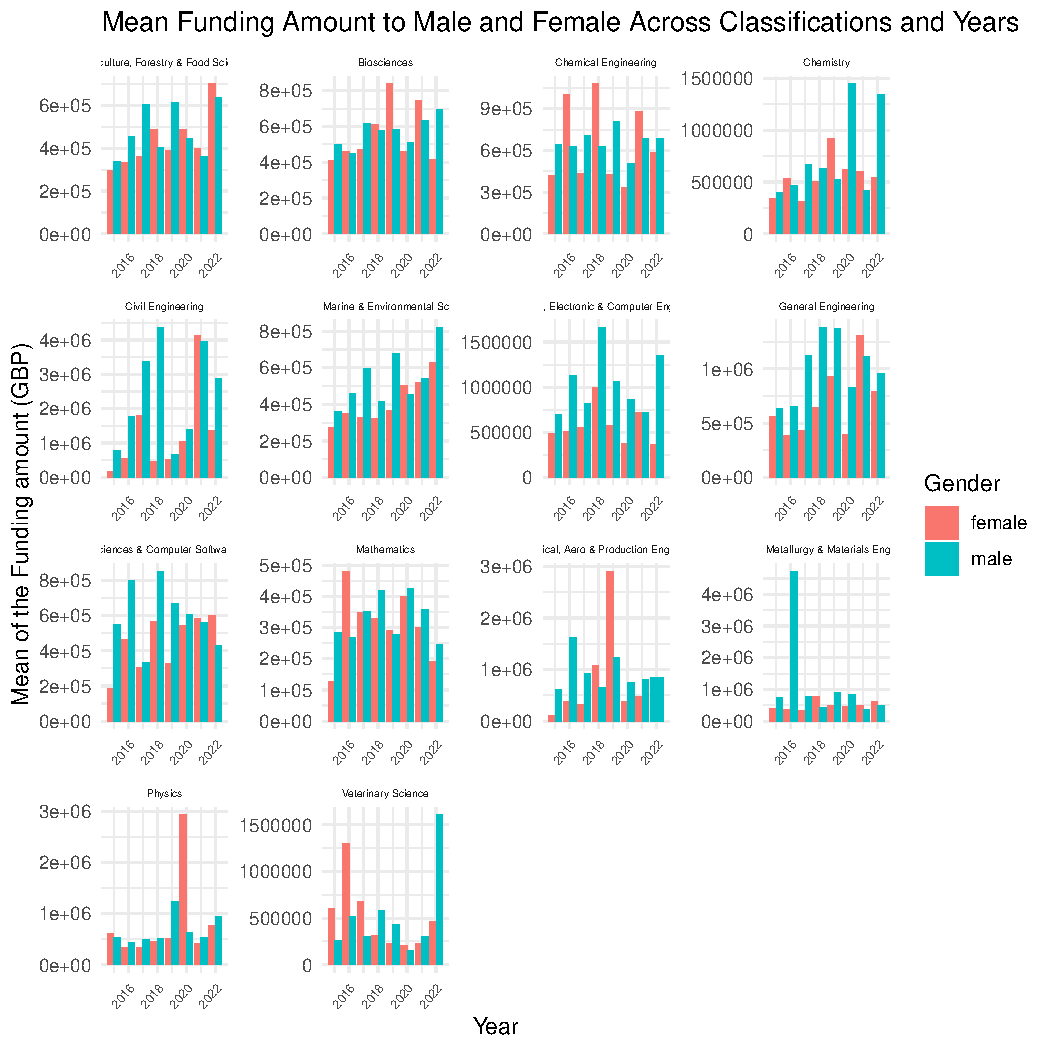
\includegraphics[width = 1\textwidth]{overleaf/results/funding_comparison.pdf}
    \caption{Mean funding allocated to each gender over time. We can observe that the gender gap in Chemistry increased over time; for Veterinary Science, the funding amount to female researchers was initially higher than male, and became lower in recent years. In most engineering-related subjects, there is a noticeable gender gap over time.}
\end{figure}
The findings in Figure 2 closely align with the observations from Figure 1. In particular, within the field of Physics, female researchers obtained a higher average funding compared to male researchers, primarily because of the markedly increased funding for women in 2020. During other years, males typically received more funding, or the funding amounts were nearly the same.
In order to test for the gender gap, hypothesis testing is required. The figure below shows the distribution of the funding amount for female researchers and male researchers. We can observe that both distributions are left skewed. Given that the observations are independent, we applied Mann-Whitney U test in this study. The test evaluated the whether the mean funding for male and female researchers is equal.

\begin{figure}
	\centering
   \begin{subfigure}{0.45\textwidth}
       \centering
       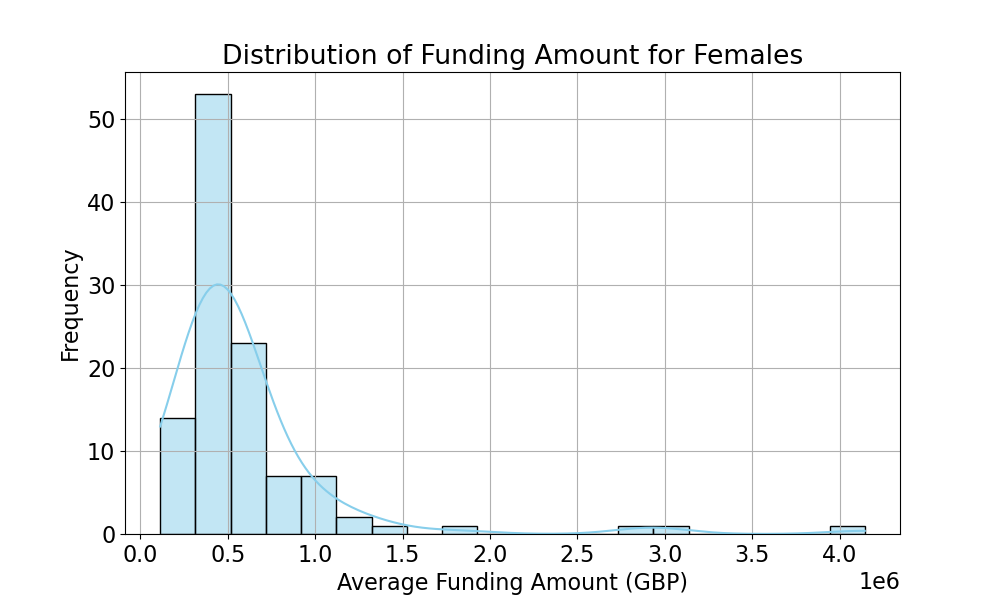
\includegraphics[width=\linewidth]{overleaf/results/female_funding_distribution.png}
   \end{subfigure}
   \begin{subfigure}{0.45\textwidth}
       \centering
       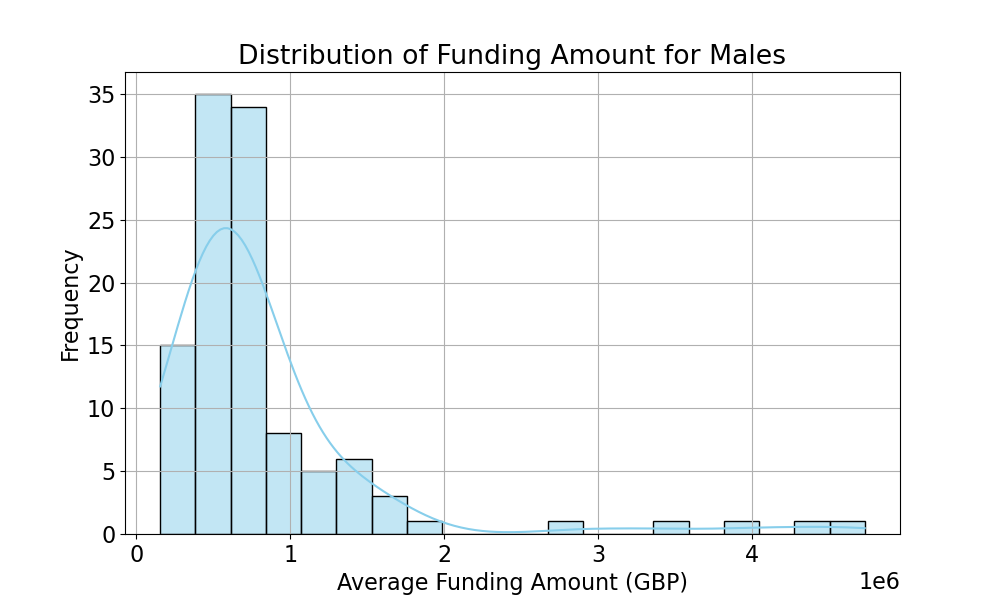
\includegraphics[width=\linewidth]{overleaf/results/male_funding_distribution.png}
   \end{subfigure}
   \caption{The distribution of average funding amount. The plots are left-skewed, meaning that a parametric test may not be a good choice.}
\end{figure}
The result of the Mann-Whitney U test shows a p-value of 1.181e-05, which is smaller than a 5\% significant level. This result indicates a highly statistically significant difference between the mean funding for male and female researchers, providing strong evident to reject the null hypothesis and to the existence of gender gap between the mean funding amount. 
 
\subsection{Comparison of the proportion of each gender getting funded}

\subsubsection{Comparison among classifications}

\begin{figure}
    \centering
    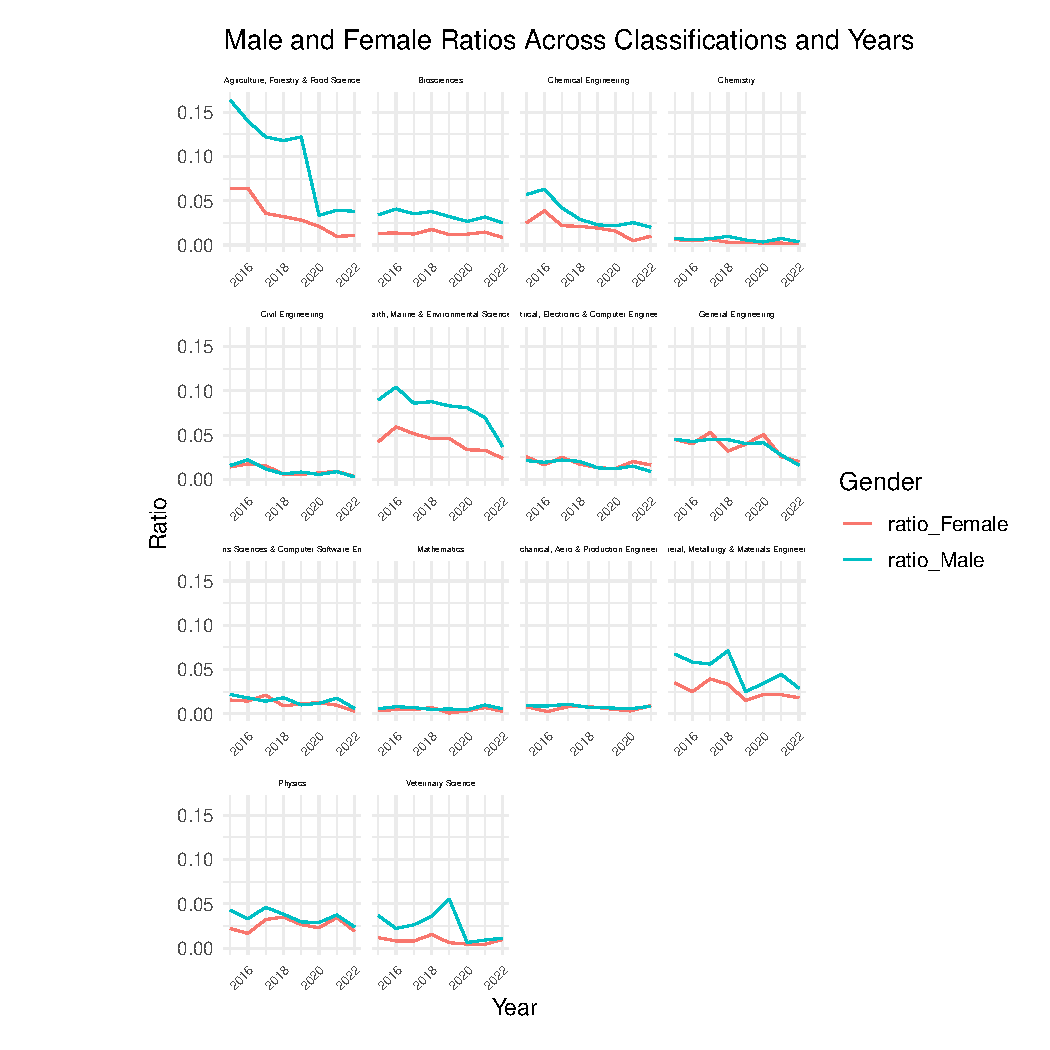
\includegraphics[width = 1\textwidth]{overleaf/results/distribution_year.pdf}
    \caption{Trends in the proportion of each gender getting funded in across categories over time. In this result, the funding proportion is calculated by dividing the funded males or females by the total number of HESA staff in each gender.}
\end{figure}


\begin{figure}
	\centering
   \begin{subfigure}{0.75\textwidth}
       \centering
       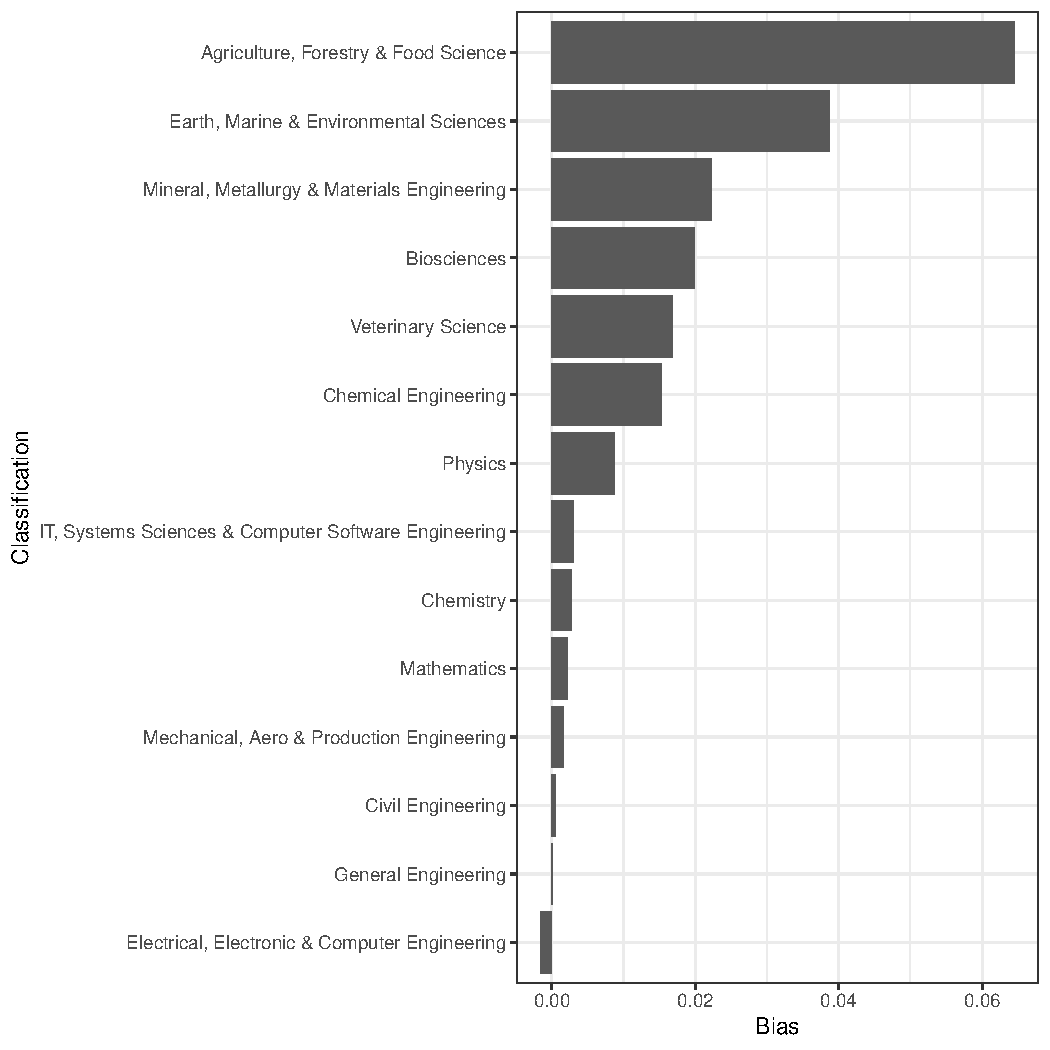
\includegraphics[width=\linewidth]{overleaf/results/rank_class.pdf}
   \end{subfigure}
   \caption{The ranking of the extent of gender bias in each classification over time. For the bias degree, I calculated the total number of funded males or females from 2015 to 2022, divided by the total number of HESA staff in the corresponding gender during the period. Then, the difference of the ratios for males and females is conducted and is reordered depending on the degree of biases - the upper represents the classification with greater gender bias.}
\end{figure}

\noindent As displayed in Figures 4 and 5, the results show a significant gender gap in the research funding of Biosciences, where the gap almost persists over time; although the extent of gender bias overall is the greatest in Agriculture, Forestry \& Food Science, the disparity has been considered to have decreased in the last few years. In contrast, there are several categories where the proportion of both genders is nearly the same over time, including General Engineering, Civil Engineering, and IT, Systems Sciences \& Computer Software Engineering. In most classifications, there is an encouraging trend indicating a reduction in the gap between men and women. An exception would be Chemistry, where the gender gap increased over time. In Electrical, Electronic \& Computer Engineering, the proportion of females funded has even surpassed that of males in recent years. Additionally, in Veterinary Science, male researchers had a higher funding ratio in the initial years, but this ratio has decreased recently, approaching that of female researchers. However, Figure 2 shows that while the average funding for males has increased in recent years, it was higher for females in earlier years. This suggests that despite female researchers receiving higher average funding, the proportion of female researchers funded has been lower compared to males.

Using a chi-square test to determine whether there is a significant difference between the funding ratios for each gender, this test is usually used to check the significance of the connection between two variables in a certain dependency relation [\cite{dura2017application}]. Specifically, the test is performed against the existence of differences in the funding ratio between male and female researchers. The result of the chi-squared test shows a p-value of 4.796e-107. Under a 5\% significance level, this result provides strong evidence to reject the null hypothesis, indicating that there is a statistically significant difference in the funding ratio between male and female researchers.

\pagebreak